% ------------------------------------------------------------------------------

Job sessions can be interactive, instead of batch (script) based. Such 
sessions can be useful for testing, debugging, and optimising code and resource 
requirements, conda or python virtual environments setup, or any likewise
preparatory work prior to batch submission.

% ------------------------------------------------------------------------------
\subsubsection{Command Line}

To request an interactive job 
%session, use, \texttt{qlogin [options]}, similarly to a 
%\tool{qsub} command-line job (e.g., \texttt{qlogin -N qlogin-test -l h\_vmem=1G}).
session, use, \texttt{salloc [options]}, similarly to a 
\tool{sbatch} command-line job, e.g.,
%
\begin{verbatim}
salloc -J interactive-test --mem=1G -p ps -n 8
\end{verbatim}
%
%Note that the options that are available for \tool{qsub} are not necessarily
%available for \tool{qlogin}, notably, \texttt{-cwd}, and, \texttt{-v}. 
%
Inside the allocated \tool{salloc} session you can run shell
commands as usual; it is recommended to use \tool{srun} for
the heavy compute steps inside \tool{salloc}.
%
If it is a quick a short job just to compile something, e.g., on
a GPU node you can use an interactive \tool{srun} directly
(note no \tool{srun} can run within \tool{srun}), e.g., a 1 hour
allocation:

For \tool{tcsh}:
\begin{verbatim}
srun --pty -n 8 -p pg --gpus=1 --mem=1Gb -t 60 /encs/bin/tcsh
\end{verbatim}

For \tool{bash}:
\begin{verbatim}
srun --pty -n 8 -p pg --gpus=1 --mem=1Gb -t 60 /encs/bin/bash
\end{verbatim}

% ------------------------------------------------------------------------------
\subsubsection{Graphical Applications}

If you need to run an on-Speed graphical-based UI application (e.g., MALTLAB,
Abaqus CME, etc.), or an IDE (PyCharm, VSCode, Eclipse)
to develop and test your job's code interactively you need to enable
X11-forwarding from your client machine to speed then to the compute node.
To do so:

\begin{enumerate}
\item
you need to run an X server on your client machine, such as,
\begin{itemize}
\item on Windows: MobaXterm with X turned on, or Xming + PuTTY with X11 forwarding, or XOrg under Cygwin
\item on macOS: XQuarz -- use its \tool{xterm} and \texttt{ssh -X}
\item on Linux just use \texttt{ssh -X speed.encs.concordia.ca} 
\end{itemize}

See \url{https://www.concordia.ca/ginacody/aits/support/faq/xserver.html}
for details.

\item
verify your X connection was properly forwarded by printing the \api{DISPLAY} variable:

\verb+echo $DISPLAY+
If it has no output, then your X forwarding is not on and you may need to re-login to Speed.

\item
Use the \option{--x11} with \tool{salloc} or \tool{srun}:

\verb+salloc ... --x11=first ...+

\item
Once landed on a compute node, verify \api{DISPLAY} again.

\item
While running under scheduler, create a run-user directory and set the variable \api{XDG\_RUNTIME\_DIR}.
\begin{verbatim}
mkdir -p /speed-scratch/$USER/run-dir
setenv XDG_RUNTIME_DIR /speed-scratch/$USER/run-dir
\end{verbatim}

\item
Launch your graphical application:

\texttt{module load} the required version, then
\tool{matlab}, or \tool{abaqus cme}, etc.
\end{enumerate}

Here's an example of starting PyCharm (see \xf{fig:pycharm}), of which we made a sample local installation.
You can make a similar install under your own directory. If using VSCode, it's
currently only supported with the \tool{--no-sandbox} option. \newline

BASH version:

\scriptsize
\begin{verbatim}
bash-3.2$ ssh -X speed (XQuartz xterm, PuTTY or MobaXterm have X11 forwarding too)
serguei@speed's password: 
[serguei@speed-submit ~] % echo $DISPLAY
localhost:14.0
[serguei@speed-submit ~] % salloc -p ps --x11=first --mem=4Gb -t 0-06:00 
bash-4.4$ echo $DISPLAY
localhost:77.0
bash-4.4$ hostname
speed-01.encs.concordia.ca
bash-4.4$ export XDG_RUNTIME_DIR=/speed-scratch/$USER/run-dir
bash-4.4$ /speed-scratch/nag-public/bin/pycharm.sh
\end{verbatim}
\normalsize

TCSH version:
\scriptsize
\begin{verbatim}
ssh -X speed (XQuartz xterm, PuTTY or MobaXterm have X11 forwarding too)
[speed-submit] [/home/c/carlos] > echo $DISPLAY
localhost:14.0
[speed-submit] [/home/c/carlos] > cd /speed-scratch/$USER
[speed-submit] [/speed-scratch/carlos] > echo $DISPLAY
localhost:13.0
[speed-submit] [/speed-scratch/carlos] > salloc -pps --x11=first --mem=4Gb -t 0-06:00
[speed-07] [/speed-scratch/carlos] > echo $DISPLAY
localhost:42.0
[speed-07] [/speed-scratch/carlos] > hostname
speed-07.encs.concordia.ca
[speed-07] [/speed-scratch/carlos] > setenv XDG_RUNTIME_DIR /speed-scratch/$USER/run-dir
[speed-07] [/speed-scratch/carlos] > /speed-scratch/nag-public/bin/pycharm.sh
\end{verbatim}
\normalsize


\begin{figure}[htpb]
			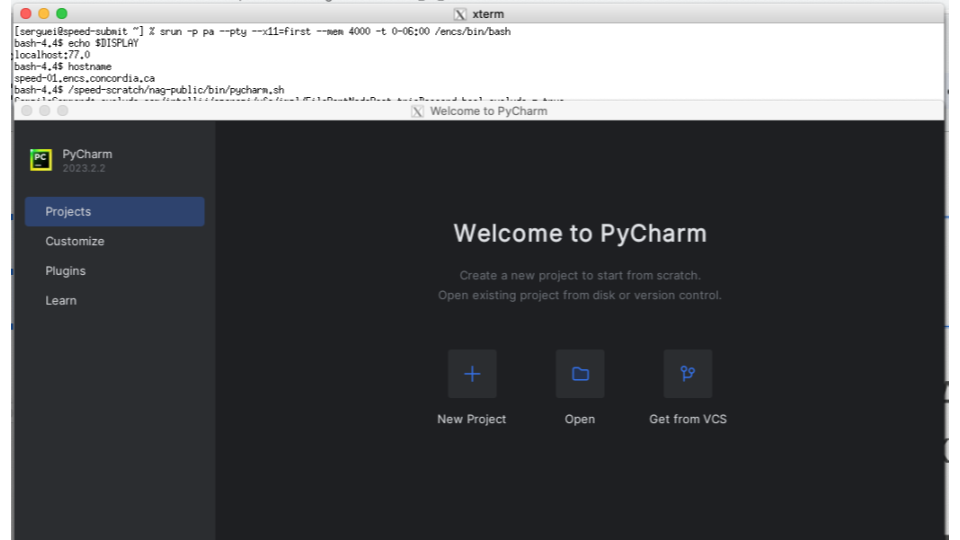
\includegraphics[width=\columnwidth]{images/pycharm}
		\caption{PyCharm Starting up on a Speed Node}
	\label{fig:pycharm}
\end{figure}

% ------------------------------------------------------------------------------
\subsubsection{Jupyter Notebooks in Singularity}
\label{sect:jupyter}

This is an example of running Jupyter notebooks together with Singularity
(more on Singularity see \xs{sect:singularity-containers}).
Here we are using one of the OpenISS-derived containers (see \xs{sect:openiss-examples} as well).

\begin{enumerate}
\item
Use the \option{--x11} with \tool{salloc} or \tool{srun} as described in the above example

\item
Load Singularity module
\verb+module load singularity/3.10.4/default+

\item
Execute this Singularity command on a single line. It's best to save it in a shell script
that you could call, since it's long.
\scriptsize
\begin{verbatim}
srun singularity exec -B $PWD\:/speed-pwd,/speed-scratch/$USER\:/my-speed-scratch,/nettemp \
 --env SHELL=/bin/bash --nv /speed-scratch/nag-public/openiss-cuda-conda-jupyter.sif \
 /bin/bash -c '/opt/conda/bin/jupyter notebook --no-browser --notebook-dir=/speed-pwd \
 --ip="*" --port=8888 --allow-root'
\end{verbatim}
\normalsize

\item
Create an \tool{ssh} tunnel between your computer and the node (\texttt{speed-XX}) where Jupyter is
running (Using \texttt{speed-submit} as a ``jump server'') (Preferably: PuTTY, see \xf{fig:putty1} and \xf{fig:putty2})
\begin{verbatim}
ssh -L 8888:speed-XX:8888 YOUR_USER@speed-submit.encs.concordia.ca
\end{verbatim}
Don't close the tunnel.

\item
Open a browser, and copy your Jupyter's token, in the screenshot
example in \xf{fig:jupyter}; each time the token will be different,
as it printed to you in the terminal.

\small
\begin{verbatim}
http://localhost:8888/?token=5a52e6c0c7dfc111008a803e5303371ed0462d3d547ac3fb
\end{verbatim}
\normalsize

\item
Work with your notebook.

\end{enumerate}

\begin{figure}[htbp]
		\centering
		\fbox{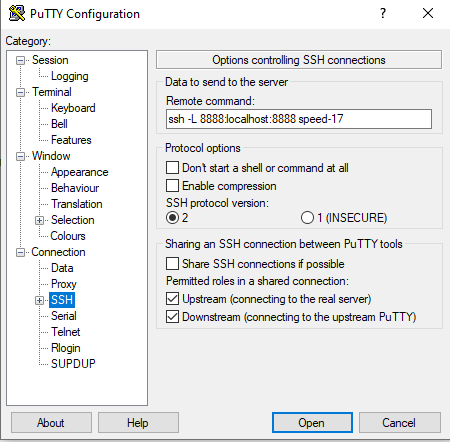
\includegraphics{images/putty1}}
	\caption{SSH tunnel configuration 1}
	\label{fig:putty1}
\end{figure}

\begin{figure}[htbp]
		\centering
		\fbox{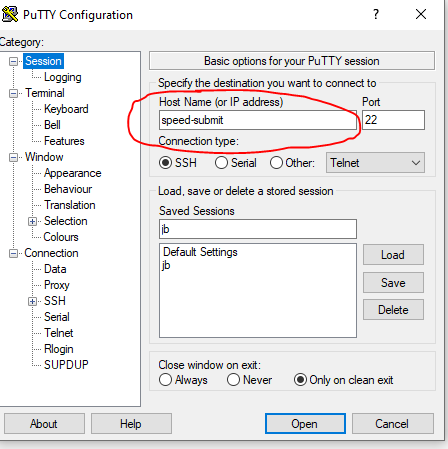
\includegraphics{images/putty2}}
	\caption{SSH tunnel configuration 2}
	\label{fig:putty2}
\end{figure}

\begin{figure}[htbp]
	\centering
	\fbox{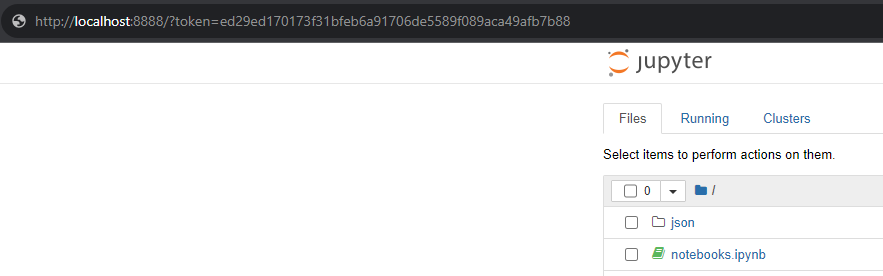
\includegraphics[width=1.00\textwidth]{images/jupyter.png}}
	\caption{Jupyter running on a Speed node}
	\label{fig:jupyter}
\end{figure}

% ------------------------------------------------------------------------------
\subsubsection{Jupyter Labs in Conda and Pytorch}
\label{sect:jupiterlabs}

This is an example of Jupyter Labs running in a Conda environment, with Pytorch

\begin{itemize}
\item
Environment preparation: for the FIRST time:
\begin{enumerate}
\item
Go to your speed-scratch directory: \texttt{cd /speed-scratch/\$USER}
\item
Create a Jupyter (name of your choice) directory: \texttt{mkdir -p Jupyter}
\item
Go to Jupyter: \texttt{cd Jupyter}
\item
Open an Interactive session: \texttt{salloc --mem=50G --gpus=1 -ppg} (or -ppt)
\item
Set env. variables, conda environment, jupyter+pytorch installation
\scriptsize
\begin{verbatim}
module load anaconda3/2023.03/default
setenv TMPDIR /speed-scratch/$USER/tmp
setenv TMP /speed-scratch/$USER/tmp
setenv CONDA_PKGS_DIRS /speed-scratch/$USER/Jupyter/pkgs 
conda create -p /speed-scratch/$USER/Jupyter/jupyter-env 
conda activate /speed-scratch/$USER/Jupyter/jupyter-env
conda install -c conda-forge jupyterlab
pip3 install torch torchvision torchaudio --index-url https://download.pytorch.org/whl/cu118
exit
\end{verbatim}
\normalsize
\end{enumerate}
\item
Running Jupyter Labs, from \textbf{speed-submit}:
\begin{enumerate}
\item
Open an Interactive session: \texttt{salloc --mem=50G --gpus=1 -ppg} (or -ppt)
\scriptsize
\begin{verbatim}
cd /speed-scratch/$USER/Jupyter
module load anaconda3/2023.03/default
setenv TMPDIR /speed-scratch/$USER/tmp
setenv TMP /speed-scratch/$USER/tmp
setenv CONDA_PKGS_DIRS /speed-scratch/$USER/Jupyter/pkgs
conda activate /speed-scratch/$USER/Jupyter/jupyter-env
jupyter lab --no-browser --notebook-dir=$PWD --ip="*" --port=8888 --port-retries=50
\end{verbatim}
\normalsize
\item
Verify which port the system has assigned to Jupyter: 
\texttt{http://localhost:XXXX/lab?token=}
\item
SSH Tunnel creation: similar to Jupyter in Singularity, see \xs{sect:jupyter}
\item
Open a browser and type: \texttt {localhost:XXXX} (port assigned)
\end{enumerate}
\end{itemize}

% ------------------------------------------------------------------------------
\subsubsection{Jupyter Labs + Pytorch in Python venv}
\label{sect:jupiterlabs-venv}

This is an example of Jupyter Labs running in a Python Virtual environment (venv), with Pytorch

\begin{itemize}
\item
Environment preparation: for the FIRST time:
\begin{enumerate}
\item
Go to your speed-scratch directory: \texttt{cd /speed-scratch/\$USER}
\item
Open an Interactive session: \texttt{salloc --mem=50G --gpus=1 --constraint=el9}
\item
Create Python venv and install jupyterlab+pytorch
\scriptsize
\begin{verbatim}
module load python/3.11.5/default
setenv TMPDIR /speed-scratch/$USER/tmp
setenv TMP /speed-scratch/$USER/tmp
setenv PIP_CACHE_DIR /speed-scratch/$USER/tmp/cache
python -m venv /speed-scratch/$USER/tmp/jupyter-venv
source /speed-scratch/$USER/tmp/jupyter-venv/bin/activate.csh
pip install jupyterlab
pip3 install torch torchvision torchaudio --index-url https://download.pytorch.org/whl/cu118
exit
\end{verbatim}
\normalsize
\end{enumerate}
\item
Running Jupyter Labs, from \textbf{speed-submit}:
\begin{enumerate}
\item
Open an Interactive session: \texttt{salloc --mem=50G --gpus=1 --constraint=el9} 
\scriptsize
\begin{verbatim}
cd /speed-scratch/$USER
module load python/3.11.5/default
setenv PIP_CACHE_DIR /speed-scratch/$USER/tmp/cache
source /speed-scratch/$USER/tmp/jupyter-venv/bin/activate.csh
jupyter lab --no-browser --notebook-dir=$PWD --ip="0.0.0.0" --port=8888 --port-retries=50
\end{verbatim}
\normalsize
\item
Verify which port the system has assigned to Jupyter: 
\texttt{http://localhost:XXXX/lab?token=}
\item
SSH Tunnel creation: similar to Jupyter in Singularity, see \xs{sect:jupyter}
\item
Open a browser and type: \texttt {localhost:XXXX} (port assigned)
\end{enumerate}
\end{itemize}


% ------------------------------------------------------------------------------
\subsubsection{VScode}
\label{sect:vscode}

This is an example of running VScode, it's similar to Jupyter notebooks, but it doesn't use containers.
This a Web version, it exists the local(workstation)-remote(speed-node) version too, but it is for Advanced users (no support, execute it at your own risk).

\begin{itemize}
\item
Environment preparation: for the FIRST time:
\begin{enumerate}
\item
Go to your speed-scratch directory: \texttt{cd /speed-scratch/\$USER}
\item
Create a vscode directory: \texttt{mkdir vscode}
\item
Go to vscode: \texttt{cd vscode}
\item
Create home and projects: \texttt {mkdir \{home,projects\}}
\item
Create this directory: \texttt {mkdir -p /speed-scratch/\$USER/run-user}
\end{enumerate}
\item
Running VScode
\begin{enumerate}
\item 
Go to your vscode directory: \texttt{cd /speed-scratch/\$USER/vscode}
\item
Open interactive session: \texttt {salloc --mem=10Gb --constraint=el9}
\item
Set environment variable: \texttt {setenv XDG\_RUNTIME\_DIR /speed-scratch/\$USER/run-user}
\item 
Run VScode, change the port if needed.
\scriptsize
\begin{verbatim}
/speed-scratch/nag-public/code-server-4.22.1/bin/code-server --user-data-dir=$PWD\/projects \
--config=$PWD\/home/.config/code-server/config.yaml --bind-addr="0.0.0.0:8080" $PWD\/projects
\end{verbatim}
\normalsize
\item
SSH Tunnel creation: similar to Jupyter, see \xs{sect:jupyter}
\item
Open a browser and type: \texttt {localhost:8080}
\item
If the browser asks for password: 
\begin{verbatim}
cat /speed-scratch/$USER/vscode/home/.config/code-server/config.yaml
\end{verbatim}

\end{enumerate}
\end{itemize}

\begin{figure}[htbp]
	\centering
	\fbox{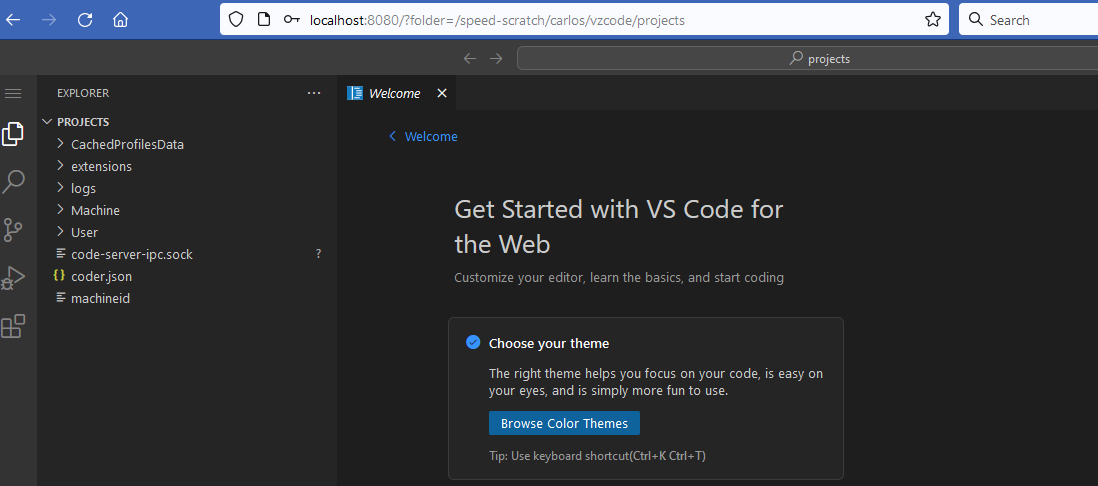
\includegraphics[width=1.00\textwidth]{images/vscode.png}}
	\caption{VScode running on a Speed node}
	\label{fig:vscode}
\end{figure}

